% Вычислительные эксперименты (1 раздел -- тестирование каждого отдельного метода на предмет скорости сходимости и качества полученного результата, можно сравнить со встроенными функциями sk-learn(?), 2 раздел -- тестирование на задаче ИАД, 3 раздел -- анализ и комментарии)

\newpage
\section{Вычислительные эксперименты}


\iffalse
Term-document matrices are used in information retrieval. Con-
sider the following selection of five documents. 1 Key words, which we call terms,
are marked in boldface.

\begin{longtable}{ l p{10cm} }
 Документ 1: & Progressive \textbf{Web} \textbf{Applications} are experiences that combine the best of the \textbf{web} and the best of \textbf{applications}. \\
 Документ 2: & The number of \textbf{transactions} in the Bitcoin \textbf{blockchain} has reached a historical maximum.\\
 Документ 3: & The reason why the Progressive \textbf{Web} \textbf{Applications} ecosystem of \textbf{tooling} seems overwhelming is because it’s always explained in the wrong \textbf{order}.\\
 Документ 4: & PayPal made the first \textbf{investment} in a \textbf{startup} working with \textbf{blockchain} \textbf{technology}.\\
 Документ 5: & Belarusian \textbf{startup} released an \textbf{application} that allows you to ``try on'' new \textbf{sneakers} before you buy them.\\
 Документ 6: & The new level of \textbf{quality} allows Progressive \textbf{Web} \textbf{Applications} to earn a place on the user's \textbf{home} screen. \\
\end{longtable}



\begin{center}
 \begin{tabular}{ l | c c c c c c }
 Term        & Док 1 & Док 2 & Док 3 & Док 4 & Док 5 & Док 6 \\
 \hline
 home        & 0 & 0 & 0 & 0 & 0 & 1 \\
 web         & 2 & 0 & 1 & 0 & 0 & 1 \\
 tool        & 0 & 0 & 1 & 0 & 0 & 0 \\
 order       & 0 & 0 & 0 & 0 & 0 & 0 \\
 investment  & 0 & 0 & 0 & 1 & 0 & 0 \\
 startup     & 0 & 0 & 0 & 1 & 1 & 0 \\
 transaction & 0 & 1 & 0 & 0 & 0 & 0 \\
 technology  & 0 & 0 & 0 & 1 & 0 & 0 \\
 application & 2 & 0 & 1 & 0 & 1 & 1 \\
 sneaker     & 0 & 0 & 0 & 0 & 1 & 0 \\
 quality     & 0 & 0 & 0 & 0 & 0 & 1 \\
 blockchain  & 0 & 1 & 0 & 1 & 0 & 0 \\
\end{tabular}
\end{center}
\fi

Терм-документная матрица представляет собой матрицу, описывающую частоту терминов, которые встречаются в коллекции документов. Такие матрицы используются при поиске информации. Рассмотрим следующую подборку из пяти документов \cite{elden}. Ключевые слова, которые мы называем терминами,
выделены жирным шрифтом.

\begin{longtable}{ l p{12cm} }
 Документ 1: & The \textbf{Google} \textbf{matrix} $P$ is a model of the \textbf{Internet}. \\
 Документ 2: & $P_{ij}$ is nonzero if there is a \textbf{link} from \textbf{Web} \textbf{page} $j$ to $i$.\\
 Документ 3: & The \textbf{Google} \textbf{matrix} is used to \textbf{rank} all \textbf{Web} \textbf{pages}.\\
 Документ 4: & The \textbf{ranking} is done by solving a \textbf{matrix} \textbf{eigenvalue} problem.\\
 Документ 5: & \textbf{England} dropped out of the top 10 in the \textbf{FIFA} \textbf{ranking}.\\
\end{longtable}

Если мы посчитаем частоту терминов встречающихся в каждом документе, мы получим следующий результат:

\begin{center}
 \begin{tabular}{ l | c c c c c c }
 Термин      & Док 1 & Док 2 & Док 3 & Док 4 & Док 5 \\
 \hline
 eigenvalue  & 0 & 0 & 0 & 1 & 0 \\
 England     & 0 & 0 & 0 & 0 & 1 \\
 FIFA        & 0 & 0 & 0 & 0 & 1 \\
 Google      & 1 & 0 & 1 & 0 & 0 \\
 Internet    & 1 & 0 & 0 & 0 & 0 \\
 link        & 0 & 1 & 0 & 0 & 0 \\
 matrix      & 1 & 0 & 1 & 1 & 0 \\
 page        & 0 & 1 & 1 & 0 & 0 \\
 rank        & 0 & 0 & 1 & 1 & 1 \\
 Web         & 0 & 1 & 1 & 0 & 0 \\
\end{tabular}
\end{center}


\newpage


Каждый документ можно представить в виде вектора из пространства $\mathbb{R}^{10}$. Составим из этих векторов матрицу. Ниже приведён полученный результат в виде матрицы $A$:
$$
A =
\begin{pmatrix}
0 & 0 & 0 & 1 & 0 \\
0 & 0 & 0 & 0 & 1 \\
0 & 0 & 0 & 0 & 1 \\
1 & 0 & 1 & 0 & 0 \\
1 & 0 & 0 & 0 & 0 \\
0 & 1 & 0 & 0 & 0 \\
1 & 0 & 1 & 1 & 0 \\
0 & 1 & 1 & 0 & 0 \\
0 & 0 & 1 & 1 & 1 \\
0 & 1 & 1 & 0 & 0
\end{pmatrix}
$$

Теперь вычислим положительную факторизацию ранга $k=3$ для данной матрицы.

\newpage


\section{Результат}

График показывает зависимость $f(W, H)$ от номера итерации.

\begin{figure}[h]
  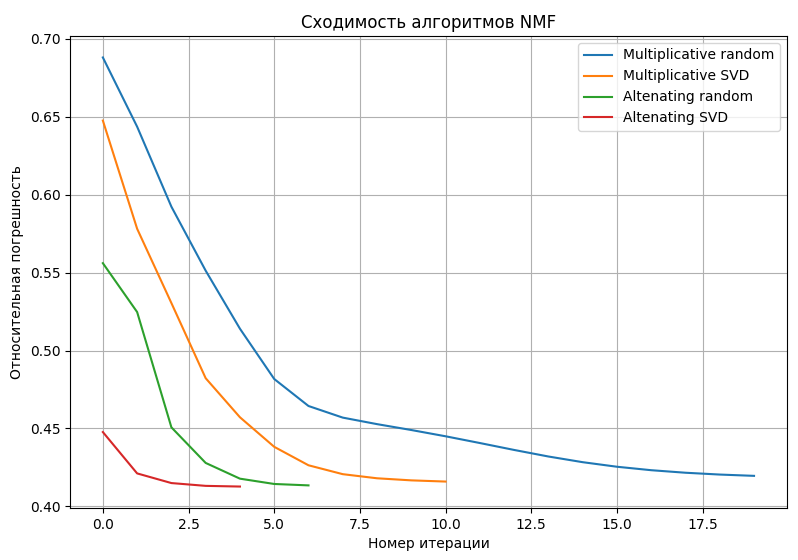
\includegraphics[width=\linewidth]{assets/Graph1.png}
  \caption{График относительной погрешности}
  \label{fig:relativeApproximationError}
\end{figure}

На Рис.~\ref{fig:relativeApproximationError} отчётливо видно, что мультипликативным алогритмам необходимо в 2-3 раза больше итераций, чтобы добиться заданной точности. Также график показывает, что мультипликативные алгоритмы чаще сходятся к более ``плохой'' точке локального минимума, которая даёт меньшую точность разложения. Касательно алгоритмов попеременных наименьших квадратов видно, что даже после первой итерации относительная ошибка значительно меньше чем у предыдущих алгоритмов и в целом они требуют намного меньше итераций.

В обоих случаях инициализация матриц $W$ и $H$ с помощью сингулярного разложения понижает ошибку на первой итерации и уменьшает количество итерации.


\newpage


Ниже приведены данные показывающие затраты по времени на выполнение алгоритмов:

\verbatimfont{\small}
\begin{verbatim}
# Initialization:
Random takes 2.002e-05s
SVD takes 4.435e-04s
# Methods:
Multiplicative random takes 3.202e-03s
Multiplicative SVD takes 6.939e-04s
Altenating random takes 1.151e-02s
Altenating SVD takes 6.742e-03s
\end{verbatim}

Ниже приведени результаты алгоритма попеременных наименьших квадратов с использованием SVD инициализации:

\begin{align*}
W H =
\begin{pmatrix}
     0.153  &   0  &   0.089 \\
     0  &   0  &   0.518 \\
     0  &   0  &   0.518 \\
     0.372  &   0.099  &   0 \\
     0.237  &   0  &   0 \\
     0  &   0.516  &   0 \\
     0.525  &  	0  &   0.027 \\
     0.042  &   0.752  &   0 \\
     0.229  &   0.131  &   0.613 \\
     0.042  &   0.752  &   0
\end{pmatrix}
\begin{pmatrix}
     2.152  &   0  &   1.897  &   1.530  &  0 \\
     0  &   1.472  &   1.022  &   0  &   0 \\
     0  &   0  &   0.250  &   0.493  &   1.844
\end{pmatrix}
\end{align*}

 Представим полученные данные в виде таблиц:

\begin{center}
 \begin{tabular}{ l | c c c c c c }
 Термин      & 1 & 2 & 3 \\
 \hline
 eigenvalue  & 0.153  &   0  &   0.089 \\
 England     & 0  &   0  &   0.518 \\
 FIFA        & 0  &   0  &   0.518 \\
 Google      & 0.372  &   0.099  &   0 \\
 Internet    & 0.237  &   0  &   0 \\
 link        & 0  &   0.516  &   0 \\
 matrix      & 0.525  &  	0  &   0.027 \\
 page        & 0.042  &   0.752  &   0 \\
 rank        & 0.229  &   0.131  &   0.613 \\
 Web         & 0.042  &   0.752  &   0
\end{tabular}
\end{center}

\begin{center}
 \begin{tabular}{ l | c c c c c c }
 Вектор      & Док 1 & Док 2 & Док 3 & Док 4 & Док 5 \\
 \hline
 1           & 2.152  &   0  &   1.897  &   1.530  &  0 \\
 2           & 0  &   1.472  &   1.022  &   0  &   0 \\
 3           & 0  &   0  &   0.250  &   0.493  &   1.844 \\
\end{tabular}
\end{center}


Напомним, что первые четыре документа рассказывают о Google и рейтинге веб-страниц, а пятый касается футбола. Из таблиц можно увидеть, что первые четыре документа представлены векторами, которые имеют большие компоненты для ключевых слов, связанных с Google. В отличие от этого, пятый документ представлен только третьим базисным вектором, так же с большой компонентой. Мы видим, что третий вектор представляет документы рассказывающие о футболе, а два других показывают документы, связанные с Google.
